%!TEX TS-program = xelatex
\documentclass[]{friggeri-cv}
\usepackage{afterpage}
\usepackage{hyperref}
\usepackage{color}
\usepackage{xcolor}
\hypersetup{
    pdftitle={},
    pdfauthor={},
    pdfsubject={},
    pdfkeywords={},
    colorlinks=false,       % no lik border color
   	allbordercolors=white,    % white border color for all
   	pdfborder=0 % Avoid cutting a piece of start character
}
\addbibresource{bibliography.bib}
\RequirePackage{xcolor}
\definecolor{pblue}{HTML}{0395DE}

\begin{document}
\header{Luca}{Olivieri}
      {Robotics Engineer}
      
% Fake text to add separator      
\fcolorbox{white}{gray}{\parbox{\dimexpr\textwidth-2\fboxsep-2\fboxrule}{%
.....
}}

% In the aside, each new line forces a line break
\begin{aside}
  \section{Contacts}    
	+39 349 28 99 132
	\href{mailto:gliolivieri@live.it}{\textbf{olivieri.luca}@outlook.com}
	~	
  \section{Address}
  	Rupinaro
    16043 Chiavari GE
    Italy
    ~
  \section{Online}
    \href{http://www.olimexsmart.it}{olimexsmart.it}    
    \href{https://github.com/olimexsmart}{\textbf{Github}: olimexsmart}
    \href{https://www.instagram.com/olimexsmart/}{\textbf{IG: }@olimexsmart}
    ~
  \section{Programming}
    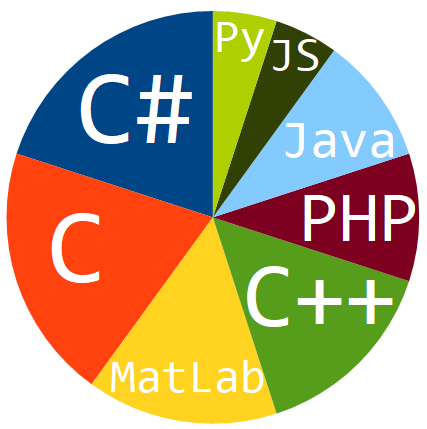
\includegraphics[scale=0.3]{img/progskilz.png}
    ~
  \section{OS Preference}
    \textbf{Unix}
\includegraphics[scale=0.40]{img/5stars.png}
    \textbf{Windows}
\includegraphics[scale=0.40]{img/4stars.png}
    \textbf{MacOS}
\includegraphics[scale=0.40]{img/1stars.png}
    ~
  \section{Languages}
    \textbf{Italian}
\includegraphics[scale=0.40]{img/5stars.png}
    \textbf{English}
\includegraphics[scale=0.40]{img/4stars.png}
    \textbf{Czech}
\includegraphics[scale=0.40]{img/1stars.png}    
\end{aside}

\section{Experience}
\begin{entrylist}
   \entry
    {2021 - now}
    {Embedded developer}
    {Hi-Lex Italy}
    {Microcontroller C programming for automotive and assembly line applications. Developing of internal tools in Python and managing of Git repositories. Assistance in electronic design.}
   \entry
	{2020 - 2021}
	{High School Teacher}
	{Natta DeAmbrosis}
	{Programming, Electronics, IT.}
  \entry
	{2019 - 2020}
	{PhD in Legged Locomotion}
	{University of Trento, Trento, Italy}
	{High performance C++ linear algebra. Optimization techniques. Publications: \textit{"Fast and Accurate Multi-Body Simulation with Stiff Viscoelastic Contacts"}. Teaching assistant in bachelor C++ programming courses. PhD interrupted at start of second year.}
  \entry
	{2019}
	{Full Stack Software Developer}
	{Deloitte Genoa}
	{Business to Business Internet of Things, both industrial and connected products. Mainly back-end in Java Spring-Boot, building microservices in Cloud Foundry environnement. Front-end with Angular. }
  \entry
    {2017}
    {Software Developer}
    {Mainsim SRL, Genoa, Italy}
    {Paid internship. Full stack web developing, database and system management. One-page application in jQuery, PHP and MySQL. Both Windows and Unix servers.}
\end{entrylist}
%\vspace{-15pt}

\section{Education}
%\vspace{-7pt}
\begin{entrylist}
  \entry
    {2016 - 2018}
    {Master's Degree in Robotics Engineering}
    {University of Genova, Genoa, Italy}
    {Modelling and control of robotic platforms, Machine Learning, Artificial Intelligence, Computer Vision, ROS, POSIX. Real-Time, concurrent and embedded programming. [107/110]\\ Title and topic of the Thesis: 
    \emph{"Hybrid indoor localization for industrial AGVs. Supervisors: Prof. Fulvio Mastrogiovanni, Ing. Marco Lazzarotto.}\\ Development from the ground-up of a segmentation algorithm and an Extended Kalman Filter for an indoor localization system based on a laser scanner sensor. Development in C++ on a Unix environment.}
  \entry
    {2013 - 2016}
    {Bachelor's Degree in Electronics Engineering and Information Technology}
    {University of Genova, Genoa, Italy}
    {Main subjects: Matematics and Physics, Programming, Control Systems, Telecommunication Systems, Digital and Analog Electronics. [104/110]\\ Title and topic of the Thesis: 
    \emph{"Source Contact Graph Routing on a Nanosat network".
    Application of a deterministic source routing on a satellite network. Supervisors: Fabio Patrone, Mario Marchese.}\\ Formulation of an a-priori routing algorithm for a satellitar network. C++ with NS3 network simulation package on Unix environment. }
  \entry
    {2008 - 2013}
    {Scientific Diploma}
    {Liceo Scientifico Marconi, Chiavari, Italy}
    {Scientific Secondary School.\\
    Main subjects: Matematics, Physics, Chemistry, Latin.}
\end{entrylist}

\clearpage
\section{Key Skills and Interests}
	%\vspace{-7pt}
	Programming in general is my first interest, constantly challenging myself with new ideas and projects. My programming projects range from high level GUI application like an Android app (Olmaredo Stego) to  embedded projects like an OBD2 telemetry interface for cars. 
	
	Electronics is my second interest, preferably digital than analog. More in detail, I developed several complex Arduino projects and experimented with the STM32 microcontroller ecosystem.
	
	During my internship at Mainsim I learned web developing, mainly back-end but a with a touch of front-end too. This new set of skills allowed me to dive into the IoT paradigm with a series of recent projects. 
	
	
\section{Personal Projects}
\begin{entrylist}
	\entry
	{2018}
	{Front Door Opener}
	{}
	{Embedded system connected to the Internet serving a login page. Upon a successful login, the front entrance of the building is opened. This allows guest to enter by themselves or enables owners to simply enter without searching  for the key. Complete with an administrator page and logs. Custom-built board.}
	\entry
	{2018}
	{Boat Tracker}
	{}
	{A self-contained embedded system used to log the position of a boat through GPS. Data is sent to a server using GSM/GPRS communication. A comprehensive web page displays the paths logged.}
	\entry
	{2018}
	{vabbuo.it}
	{}
	{A web site that allows users to post random thoughts. The idea is that is then used as a community-fed living wallpaper. Exercise for full-stack web programming.}
	\entry	
	{2017}
	{Beating Sign}
	{}
	{Home decoration that lights up following the heart rhythm of the user on the previous day. A server retrieves heart rate information from Fitbit server using the OAuth2 protocol. The object is connected trough Wi-Fi and periodically asks for data to the server.}	
	\entry
	{2016}
	{Olmaredo Stego}
	{}
	{Free Android application that implements image spread-spectrum steganography. In short it allows the user to embed text messages in photos that can be retrieved trough a password.}
	\entry
	{2015}
	{OBD2 Console}
	{}
	{An embedded system connects through bluetooth to an OBD2 adapter present on the car and displays information about the state of the engine on its screens.}	
\end{entrylist}
	
\clearpage
\section{Other Info}
\vspace{-7pt}
\begin{itemize}
	\itemsep-0.4em
	\item Proficient with \LaTeX\ , Creo PTC CAD, Simulink and Git
	\item Tin soldering through-hole and some SMD
	\item English language PET and First certificates
	\item Knowledge and interest in digital photography
	\item European driving license for cars and bikes	
	\item Capable clerk in family-run hardware store	
\end{itemize}

\section{Disclaimer}
Acconsento alla pubblicazione del mio CV in ottemperanza alle disposizioni di legge dettate in materia di trasparenza (D.Lgs. 33/2013).

\begin{flushleft}
\emph{February 25th, 2021}
\end{flushleft}
\begin{flushright}
\emph{Luca Olivieri}
\end{flushright}

%%% This piece of code has been commented by Karol Kozioł due to biblatex errors. 
% 
%\printbibsection{article}{article in peer-reviewed journal}
%\begin{refsection}
%  \nocite{*}
%  \printbibliography[sorting=chronological, type=inproceedings, title={international peer-reviewed conferences/proceedings}, notkeyword={france}, heading=subbibliography]
%\end{refsection}
%\begin{refsection}
%  \nocite{*}
%  \printbibliography[sorting=chronological, type=inproceedings, title={local peer-reviewed conferences/proceedings}, keyword={france}, heading=subbibliography]
%\end{refsection}
%\printbibsection{misc}{other publications}
%\printbibsection{report}{research reports}

\end{document}
